\documentclass[8pt,aspectratio=169]{beamer}
\usetheme{Madrid}
\usepackage{graphicx}
\usepackage{booktabs}
\usepackage{adjustbox}
\usepackage{multicol}
\usepackage{amsmath}
\usepackage{amssymb}
\usepackage{tikz}
\usepackage{hyperref}
\usepackage{algorithm}
\usepackage{algorithmic}
\usepackage{colortbl}
\usepackage{pgfplots}
\pgfplotsset{compat=1.18}

% TikZ libraries for comics, diagrams, stakeholder maps
\usetikzlibrary{arrows.meta,positioning,shapes.callouts,shapes.geometric,decorations.pathreplacing}

% Color definitions
\definecolor{mlblue}{RGB}{0,102,204}
\definecolor{mlpurple}{RGB}{51,51,178}
\definecolor{mllavender}{RGB}{173,173,224}
\definecolor{mllavender2}{RGB}{193,193,232}
\definecolor{mllavender3}{RGB}{204,204,235}
\definecolor{mllavender4}{RGB}{214,214,239}
\definecolor{mlorange}{RGB}{255, 127, 14}
\definecolor{mlgreen}{RGB}{44, 160, 44}
\definecolor{mlred}{RGB}{214, 39, 40}
\definecolor{mlgray}{RGB}{127, 127, 127}
\definecolor{lightgray}{RGB}{240, 240, 240}
\definecolor{midgray}{RGB}{180, 180, 180}

% NEW COLORS for mini-lecture
\definecolor{dfteal}{RGB}{0,128,128}
\definecolor{dfred}{RGB}{180,30,30}

% Backward compatibility
\colorlet{MLPurple}{mlpurple}
\colorlet{MLBlue}{mlblue}
\colorlet{MLOrange}{mlorange}
\colorlet{MLGreen}{mlgreen}
\colorlet{MLRed}{mlred}
\colorlet{MLLavender}{mllavender}
\colorlet{MLGray}{mlgray}

% Theme colors (exact Madrid settings)
\setbeamercolor{palette primary}{bg=mllavender3,fg=mlpurple}
\setbeamercolor{palette secondary}{bg=mllavender2,fg=mlpurple}
\setbeamercolor{palette tertiary}{bg=mllavender,fg=white}
\setbeamercolor{palette quaternary}{bg=mlpurple,fg=white}
\setbeamercolor{structure}{fg=mlpurple}
\setbeamercolor{section in toc}{fg=mlpurple}
\setbeamercolor{subsection in toc}{fg=mlblue}
\setbeamercolor{title}{fg=mlpurple}
\setbeamercolor{frametitle}{fg=mlpurple,bg=mllavender3}
\setbeamercolor{block title}{bg=mllavender2,fg=mlpurple}
\setbeamercolor{block body}{bg=mllavender4,fg=black}
\setbeamertemplate{navigation symbols}{}
\setbeamertemplate{itemize items}[circle]
\setbeamertemplate{enumerate items}[default]
\setbeamersize{text margin left=5mm,text margin right=5mm}

% Footer
\setbeamertemplate{footline}{
  \leavevmode%
  \hbox{%
    \begin{beamercolorbox}[wd=.333333\paperwidth,ht=2.25ex,dp=1ex,center]{author in head/foot}%
      \usebeamerfont{author in head/foot}Methods and Algorithms
    \end{beamercolorbox}%
    \begin{beamercolorbox}[wd=.333333\paperwidth,ht=2.25ex,dp=1ex,center]{title in head/foot}%
      \usebeamerfont{title in head/foot}MSc Data Science
    \end{beamercolorbox}%
    \begin{beamercolorbox}[wd=.333333\paperwidth,ht=2.25ex,dp=1ex,right]{date in head/foot}%
      \usebeamerfont{date in head/foot}\insertframenumber{} / \inserttotalframenumber\hspace*{2ex}
    \end{beamercolorbox}}%
  \vskip0pt%
}

\newcommand{\bottomnote}[1]{%
\vfill
\vspace{-2mm}
\textcolor{mllavender2}{\rule{\textwidth}{0.4pt}}
\vspace{1mm}
\footnotesize
\textbf{#1}
}

\newenvironment{compactlist}{%
  \begin{itemize}%
    \setlength{\itemsep}{2pt}%
    \setlength{\parskip}{0pt}%
    \setlength{\parsep}{0pt}%
}{%
  \end{itemize}%
}

\newcommand{\highlight}[1]{\textcolor{mlorange}{\textbf{#1}}}
\newcommand{\mathbold}[1]{\boldsymbol{#1}}

\title[Decision Trees Mini-Lecture]{Decision Trees}
\subtitle{A 10-Slide Mini-Lecture}
\author{Methods and Algorithms}
\institute{MSc Data Science}
\date{}

\begin{document}

%% ================================================================
%% SLIDE 1: WHY -- TikZ Comic
%% ================================================================
\begin{frame}[t]{Why Would a Bank Let a Flowchart Decide Who Gets a Loan?}
\begin{columns}[T]
\column{0.55\textwidth}
\small
\textbf{The Dilemma}
\begin{compactlist}
\item \footnotesize Banks process \highlight{thousands of loan applications} daily
\item \footnotesize Human officers are inconsistent --- same case, different outcomes
\item \footnotesize What if we could automate decisions with a sequence of questions?
\end{compactlist}
\vspace{2mm}
\begin{block}{Punchline}
\footnotesize What if the flowchart is wrong?
\end{block}

\column{0.42\textwidth}
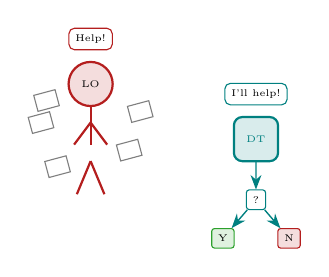
\begin{tikzpicture}[scale=0.7, every node/.style={transform shape}]
% Loan officer drowning in papers
\node[circle, draw=dfred, fill=dfred!15, minimum size=8mm, line width=0.8pt] (officer) at (0,3.5) {};
\node[font=\tiny] at (0,3.5) {LO};
\draw[dfred, line width=0.8pt] (officer.south) -- ++(0,-0.7);
\draw[dfred, line width=0.8pt] (-0.3,2.4) -- (0,2.8) -- (0.3,2.4);
\draw[dfred, line width=0.8pt] (0,2.1) -- (-0.25,1.5);
\draw[dfred, line width=0.8pt] (0,2.1) -- (0.25,1.5);
% Papers around officer
\foreach \x/\y in {-0.8/3.2, 0.9/3.0, -0.6/2.0, 0.7/2.3, -0.9/2.8} {
  \node[draw=mlgray, fill=white, minimum width=4mm, minimum height=3mm, rotate=15, font=\tiny] at (\x,\y) {};
}
\node[rounded corners=2pt, draw=dfred, fill=white, font=\tiny, above=2mm of officer] {Help!};

% Flowchart robot helping
\node[rounded corners=3pt, draw=dfteal, fill=dfteal!15, minimum width=8mm, minimum height=8mm, line width=0.8pt] (robot) at (3,2.5) {};
\node[font=\tiny, text=dfteal] at (3,2.5) {DT};
% Small flowchart inside/near robot
\node[rounded corners=1pt, draw=dfteal, fill=white, minimum width=3mm, minimum height=2mm, font=\tiny] (q1) at (3,1.4) {?};
\node[rounded corners=1pt, draw=mlgreen, fill=mlgreen!15, minimum width=3mm, minimum height=2mm, font=\tiny] (y) at (2.4,0.7) {Y};
\node[rounded corners=1pt, draw=dfred, fill=dfred!15, minimum width=3mm, minimum height=2mm, font=\tiny] (n) at (3.6,0.7) {N};
\draw[-{Stealth}, dfteal, line width=0.5pt] (q1) -- (y);
\draw[-{Stealth}, dfteal, line width=0.5pt] (q1) -- (n);
\draw[-{Stealth}, dfteal, line width=0.5pt] (robot.south) -- (q1);

\node[rounded corners=2pt, draw=dfteal, fill=white, font=\tiny, above=2mm of robot] {I'll help!};
\end{tikzpicture}
\end{columns}
\bottomnote{Decision trees automate expert judgment into a reproducible, auditable flowchart}
\end{frame}

%% ================================================================
%% SLIDE 2: FEEL -- Reflection Prompt
%% ================================================================
\begin{frame}[t]{You Are the Loan Officer --- What Questions Would You Ask?}
\begin{columns}[T]
\column{0.55\textwidth}
\small
\textbf{Think Before You Compute}

\footnotesize
Imagine you must approve or deny a loan in 30 seconds. What three questions would you ask?
\begin{compactlist}
\item \footnotesize Income above a threshold?
\item \footnotesize Employed for more than 2 years?
\item \footnotesize Credit history clean?
\end{compactlist}
\vspace{2mm}
\begin{exampleblock}{Reflection Prompt}
\footnotesize A decision tree is just a \highlight{structured sequence of questions} --- exactly what you just did intuitively.
\end{exampleblock}

\column{0.42\textwidth}
\vspace{8mm}
\fcolorbox{mlpurple}{mlpurple!10}{%
\parbox{0.9\columnwidth}{%
\footnotesize
\textcolor{mlpurple}{\textbf{Build your intuition:}} every time you triage decisions with yes/no questions, you are mentally constructing a decision tree.%
}}
\end{columns}
\bottomnote{The key insight: a DT learns \emph{which} questions to ask and \emph{in what order} from data}
\end{frame}

%% ================================================================
%% SLIDE 3: WHAT -- Plain English Definition
%% ================================================================
\begin{frame}[t]{What IS a Decision Tree?}
\small
\textbf{Plain English:} ``A flowchart that \highlight{learns which questions to ask} from data.''

\vspace{3mm}
\footnotesize
\begin{columns}[T]
\column{0.50\textwidth}
\textbf{Key Terms (no formulas)}
\begin{compactlist}
\item \footnotesize \textbf{Root:} the first question asked
\item \footnotesize \textbf{Node:} each decision point along the way
\item \footnotesize \textbf{Leaf:} the final answer (approve / deny)
\end{compactlist}

\column{0.48\textwidth}
\begin{compactlist}
\item \footnotesize \textbf{Split:} the branch that divides data into subsets
\item \footnotesize \textbf{Depth:} how many levels of questions
\item \footnotesize \textbf{Branch:} the path from root to leaf
\end{compactlist}
\end{columns}

\vspace{3mm}
\begin{block}{Insight}
\footnotesize A deeper tree asks more questions --- more specific but risks memorizing the training data.
\end{block}
\bottomnote{Decision trees are \textbf{non-parametric}: no assumed functional form, just data-driven splits}
\end{frame}

%% ================================================================
%% SLIDE 4: CASE -- One Transaction Navigates the Tree
%% ================================================================
\begin{frame}[t]{How Does One Transaction Navigate the Tree?}
\begin{columns}[T]
\column{0.50\textwidth}
\small
\textbf{Tracing a Path}

\footnotesize
Follow one loan applicant through the tree:
\begin{compactlist}
\item \footnotesize \textcolor{mlred}{Amount > \$500?} $\to$ Yes
\item \footnotesize \textcolor{mlred}{Time < 2am?} $\to$ No
\item \footnotesize \textcolor{mlred}{Foreign IP?} $\to$ Yes $\to$ \textbf{FRAUD}
\end{compactlist}
\vspace{2mm}
\begin{block}{Insight}
\footnotesize Each path from root to leaf = one interpretable decision rule.
\end{block}

\column{0.48\textwidth}
\vspace{2mm}

\includegraphics[width=\textwidth]{01_decision_tree/chart.pdf}
\end{columns}
\bottomnote{Interpretability is the single biggest advantage of decision trees over black-box models}
\end{frame}

%% ================================================================
%% SLIDE 5: HOW -- Gini Impurity
%% ================================================================
\begin{frame}[t]{How Does the Tree Decide Which Question to Ask First?}
\begin{columns}[T]
\column{0.50\textwidth}
\small
\textbf{Gini Intuition}

\footnotesize
Pick the question that creates the \highlight{purest groups}.

\vspace{1mm}
\textbf{Worked example:}
\begin{compactlist}
\item \footnotesize 100 applicants: 60 repay, 40 default (G = 0.48)
\item \footnotesize Left child: 40 apps (28/12, G = 0.42)
\item \footnotesize Right child: 60 apps (54/6, G = 0.18)
\item \footnotesize Weighted avg: $\frac{40}{100}\times 0.42 + \frac{60}{100}\times 0.18 = 0.276$
\item \footnotesize \textbf{Reduction = 0.204}
\end{compactlist}

\column{0.48\textwidth}
\vspace{2mm}

\includegraphics[width=\textwidth]{08_gini_split/chart.pdf}
\end{columns}
\bottomnote{Gini impurity measures how often a randomly chosen sample would be misclassified}
\end{frame}

%% ================================================================
%% SLIDE 6: RISK -- TikZ Comic (Overfitting)
%% ================================================================
\begin{frame}[t]{What Happens When the Tree Memorizes the Training Data?}
\begin{columns}[T]
\column{0.55\textwidth}
\small
\textbf{The Overfitting Trap}
\begin{compactlist}
\item \footnotesize A deep tree with 500 branches can memorize every training example
\item \footnotesize A new applicant arrives and the tree says: ``I've never seen THIS before!''
\item \footnotesize \highlight{A tree that memorizes can't generalize}
\end{compactlist}
\vspace{2mm}
\begin{block}{Insight}
\footnotesize Pruning (limiting depth, min samples per leaf) trades training accuracy for generalization.
\end{block}

\column{0.42\textwidth}
\begin{tikzpicture}[scale=0.65, every node/.style={transform shape}]
% Giant overfit tree
\node[circle, draw=dfred, fill=dfred!15, minimum size=6mm, line width=0.7pt] (root) at (0,4) {};
\foreach \x in {-1.5, 1.5} {
  \node[circle, draw=dfred, fill=dfred!10, minimum size=4mm] (n1\x) at (\x,3) {};
  \draw[dfred, line width=0.5pt] (root) -- (n1\x);
}
\foreach \x/\p in {-2.2/-1.5, -0.8/-1.5, 0.8/1.5, 2.2/1.5} {
  \node[circle, draw=dfred, fill=dfred!8, minimum size=3mm] (n2\x) at (\x,2) {};
  \draw[dfred, line width=0.4pt] (n1\p) -- (n2\x);
}
\foreach \x in {-2.5,-1.9,-1.1,-0.5,0.5,1.1,1.9,2.5} {
  \node[rectangle, draw=dfred, fill=dfred!5, minimum size=2mm, font=\tiny] at (\x,1.2) {};
}
\node[font=\tiny\bfseries, text=dfred] at (0,0.7) {500 branches!};

% New applicant
\node[circle, draw=mlblue, fill=mlblue!20, minimum size=6mm, line width=0.7pt] (new) at (0,-0.3) {};
\node[font=\tiny, text=mlblue] at (0,-0.3) {?};
\draw[-{Stealth}, mlblue, line width=0.6pt] (new.north) -- ++(0,0.3);

% Speech bubble
\node[rounded corners=3pt, draw=dfred, fill=white, font=\tiny, text width=2cm, align=center] at (3,1.5) {I've never seen THIS before!};
\end{tikzpicture}
\end{columns}
\bottomnote{Rule of thumb: if train accuracy $\gg$ test accuracy, your tree is too deep}
\end{frame}

%% ================================================================
%% SLIDE 7: WHERE -- Industry Applications
%% ================================================================
\begin{frame}[t]{Where Do Banks Actually Use Decision Trees?}
\small
\textbf{Industry Applications}
\begin{columns}[T]
\column{0.48\textwidth}
\begin{compactlist}
\item \footnotesize \textbf{Credit scoring:} approve/deny based on income, history, employment
\item \footnotesize \textbf{Fraud detection:} flag suspicious transactions with interpretable rules
\item \footnotesize \textbf{Anti-money laundering:} triage alerts by risk level
\end{compactlist}

\column{0.48\textwidth}
\begin{compactlist}
\item \footnotesize \textbf{Customer churn:} identify at-risk clients
\item \footnotesize \textbf{Regulatory compliance:} auditors can read every decision path
\end{compactlist}
\vspace{3mm}
\begin{block}{Bridge}
\footnotesize DTs are the \highlight{building block} inside Random Forests --- next lecture.
\end{block}
\end{columns}
\bottomnote{Regulators favor DTs because every prediction has a human-readable explanation}
\end{frame}

%% ================================================================
%% SLIDE 8: IMPACT -- Stakeholder Analysis
%% ================================================================
\begin{frame}[t]{Who Wins and Who Loses When Trees Replace Human Judgment?}
\small
\textbf{Stakeholder Analysis}
\begin{columns}[T]
\column{0.48\textwidth}
\textbf{\textcolor{mlgreen}{Winners}}
\begin{compactlist}
\item \footnotesize \textbf{Consistency:} same inputs always produce same output
\item \footnotesize \textbf{Speed:} thousands of decisions per second
\item \footnotesize \textbf{Scalability:} one trained tree serves all branches
\end{compactlist}

\column{0.48\textwidth}
\textbf{\textcolor{dfred}{Losers}}
\begin{compactlist}
\item \footnotesize \textbf{Edge cases:} unusual applicants get misclassified
\item \footnotesize \textbf{Explainability pressure:} ``why was I denied?''
\item \footnotesize \textbf{Bias risk:} tree can learn discriminatory patterns from data
\end{compactlist}
\end{columns}
\vspace{2mm}
\begin{block}{Insight}
\footnotesize Automation amplifies both the strengths and biases in historical data.
\end{block}
\bottomnote{Fair lending laws (ECOA, GDPR) require explanations for adverse decisions}
\end{frame}

%% ================================================================
%% SLIDE 9: SO WHAT -- Decision Framework
%% ================================================================
\begin{frame}[t]{When Should You Use a Single Tree --- and When Should You Not?}
\small
\textbf{Decision Framework}
\begin{columns}[T]
\column{0.48\textwidth}
\textbf{\textcolor{mlgreen}{Use a Decision Tree when:}}
\begin{compactlist}
\item \footnotesize Interpretability is required by regulators
\item \footnotesize Small to medium dataset
\item \footnotesize You need a fast first baseline
\end{compactlist}

\column{0.48\textwidth}
\textbf{\textcolor{dfred}{Don't use a single tree when:}}
\begin{compactlist}
\item \footnotesize High accuracy is critical $\to$ Random Forest
\item \footnotesize Many features $\to$ prone to overfit
\item \footnotesize Data is noisy $\to$ high variance
\end{compactlist}
\end{columns}
\vspace{2mm}
\begin{block}{Insight}
\footnotesize A single tree is a \highlight{stepping stone}: learn it well, then ensemble it.
\end{block}
\bottomnote{In practice, single trees are used for baselines and explanation; ensembles for production}
\end{frame}

%% ================================================================
%% SLIDE 10: ACT -- Exercise + Closing Comic
%% ================================================================
\begin{frame}[t]{Can You Build This Tree by Hand?}
\begin{columns}[T]
\column{0.55\textwidth}
\small
\textbf{Exercise: Build a 2-Level Tree}

\footnotesize
Given 6 loan applicants with 2 features:

\vspace{1mm}
\begin{adjustbox}{max width=\columnwidth}
\begin{tabular}{cccc}
\toprule
\textbf{ID} & \textbf{Income (\$k)} & \textbf{Credit Score} & \textbf{Repay?} \\
\midrule
1 & 80 & 720 & Yes \\
2 & 35 & 580 & No \\
3 & 60 & 650 & Yes \\
4 & 25 & 550 & No \\
5 & 90 & 700 & Yes \\
6 & 40 & 610 & No \\
\bottomrule
\end{tabular}
\end{adjustbox}

\vspace{2mm}
\begin{compactlist}
\item \footnotesize Which feature splits best at the root?
\item \footnotesize Draw the tree with 2 levels
\item \footnotesize What is the Gini at each node?
\end{compactlist}

\column{0.42\textwidth}
\vspace{2mm}
\centering
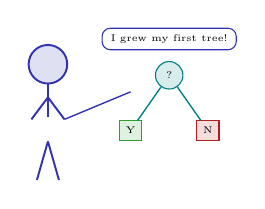
\begin{tikzpicture}[scale=0.7, every node/.style={transform shape}]
% Stick figure holding tree diagram
\node[circle, draw=mlpurple, fill=mlpurple!15, minimum size=7mm, line width=0.7pt] (head) at (0,3) {};
\draw[mlpurple, line width=0.7pt] (head.south) -- ++(0,-0.6);
\draw[mlpurple, line width=0.7pt] (-0.3,2.0) -- (0,2.4) -- (0.3,2.0);
\draw[mlpurple, line width=0.7pt] (0,1.6) -- (-0.2,0.9);
\draw[mlpurple, line width=0.7pt] (0,1.6) -- (0.2,0.9);

% Tree diagram held by figure
\node[circle, draw=dfteal, fill=dfteal!15, minimum size=4mm, font=\tiny] (t1) at (2.2,2.8) {?};
\node[rectangle, draw=mlgreen, fill=mlgreen!15, minimum size=3mm, font=\tiny] (t2) at (1.5,1.8) {Y};
\node[rectangle, draw=dfred, fill=dfred!15, minimum size=3mm, font=\tiny] (t3) at (2.9,1.8) {N};
\draw[dfteal, line width=0.5pt] (t1) -- (t2);
\draw[dfteal, line width=0.5pt] (t1) -- (t3);

% Arm pointing to tree
\draw[mlpurple, line width=0.5pt] (0.3,2.0) -- (1.5,2.5);

% Speech bubble
\node[rounded corners=3pt, draw=mlpurple, fill=white, font=\tiny, text width=2.2cm, align=center, above=2mm of t1] {I grew my first tree!};
\end{tikzpicture}
\end{columns}
\bottomnote{Hint: compute Gini for each possible split and pick the one with the largest reduction}
\end{frame}

\end{document}
